%!TEX root = ../../dissertacao.tex
This chapter~\label{chap:inductive} brings a brief introduction on formal verification and a more detailed explanation on the selected approach to be used in this work: the Inductive Method. Its syntax will be restrained for comprehension of the proposed problem.





\section{Formal Verification}
Using the previous definitions for security protocols, it is easy to perceive that one can reason about protocol rules, \textit{verifying} if they are correct with respect to the protocol's goals.

Informal reasoning on verifying protocols was the first attempt to guarantee their correctness, succeeding in recognizing some flaws and weaknesses quickly and providing a good understanding about protocols design~\cite{Bella2007}. However, not finding an error does not mean that a certain model does not hold one. Such method was failing to identify critical flaws in major security protocols, where the classical example of the Needham-Schroeder protocol~\cite{NeedhamSchroeder78} can be cited. The techniques in~\cite{Lowe96} exposed the protocol's limitations, despite the authors efforts on its specification and informal verification.

This scenario was optimal for the rise of formal verification on security protocols~\cite{Meadows96, Meadows94, Kemmerer94, Burrows90}, allowing a mathematical and profitable procedure for reasoning about abstract protocols models. Thus, it is important to emphasize that the method focus on the protocol properties and rules, and rarely on its execution.

Formal verification requires the definition of such protocols in a proper language, suitable for the application of such methods and deservedly automated through computational methods. Formal methods can be divided in two major categories, according to~\cite{BoydMathuria2008}:

\begin{itemize}
  \item \textbf{Model checking}: protocol behaviors can be modeled as a finite set of states. Such proposal is suitable for checking if a given configuration satisfy a set of correctness conditions and analyze a certain past configuration, searching for attacks attempts. This approach is more appropriate for finding inconsistencies and attacks in the protocol rather than proving its correctness;

  \item \textbf{Theorem proving}: postulating the protocol as a model, taking into account \textit{all} possible protocol behaviors, and checking its correctness through the verification of the theorem claims. This method is more suitable for proving the correctness of the protocol rather than finding possible attacks on them.
\end{itemize}

Both methods are aided by computer assistance, where theorem proving may be a less automated approach. Concerning the protocol analyzed in this document and our goal to prove its correctness, it is trivial to guess that our chosen method fits the theorem proving set.





\section{Method Introduction}\label{sec:inductive-method}
The Inductive Method aims for both formalization and verification of security protocols, being based on model checking and structural induction. First, the intended protocol \(\mathcal{P}\) must be defined as a inductively constructed model \(P\), composed by rules describing the real world steps of \(\mathcal{P}\).

An unlimited set of agents is considered, who can fire events accordingly with model \(P\), in any desired order or regularity, composing the network traffic. Agents can interleave between protocol sessions indefinitely. Among the agents, relies a special one, the Spy, who has control over the network and compromised agents, modeling the threat scenario.

At a second stage, the model is verified towards proposed properties, reasoning along technical and theoretical traits. Here, structural induction takes crucial role. If a security property must hold for the protocol, it must hold for all possible traces derived from the formal model \(P\), hence induction over the set of possible network traces is main proof tool used in this phase.

Induction has been previously used in the literature, for example in the NRL Protocol Analyzaer by C.~Meadows~\cite{Meadows96}, and the Inductive Method has similarities with other model checking theories, like CSP~\cite{RyanSchneider2010}. It comprehends a strong threat model and concurrency among peers, however it does not check liveness properties. Moreover, the framework which it is built on provides easy ways for extension, allowing steady formalizations of atypical systems, a feature which interests us.

The method was first proposed by L.~Paulson~\cite{Paulson98} and extended by G.~Bella~\cite{Bella2007} and has presented verifications for many deployed and significant protocols~\cite{Paulson99, BellaPaulson2006, Bella2003}.



\subsection{Isabelle}
Given the considerably great number of possible traces which can be derived by a model, proofs can take a substantial amount of work. As a result, the use of an automatic theorem prover is suitable, being Isabelle~\cite{isabelle} the system where the theory framework is built. Thus, the generated proofs are machine checkable, enabling a deep understanding of its anatomy and easy error maintenance.

Isabelle is a generic theorem prover, which can reason over several formal systems, in an interactive way. Hence, proofs are not entirely automatic, requiring certain user guidance. It combines high order logic, typed formalism and quantifiers for functions, predicates and sets. Also, the system has great proof tools, specially its simplifiers, induction-oriented commands and some automatic provers, offering a valuable automation for proofs.

Lemmas and theorems are stated as goals, where the user must apply proof tactics, being able to use previously proved lemmas. Such process may derive subgoals, which also need to be dealt with. If an user fails to find a proof for a certain property, this may not be a certification of proof unsatisfiability. Despite, the proof or somes of its aspects may be built on top of wrong formalizations, meaning the user is not skilled enough. Thereby, the process is arduous and must be done with care.

Each formalized theory in Isabelle is contained in a proof script. Also, each Isabelle distribution comes with a library of such formalizations. The Inductive Method framework is defined in the \textit{Auth} library~\cite{isabelle-hol-auth}, comprised in three files: \texttt{Message.thy}, \texttt{Event.thy} and \texttt{Public.thy}. These files will be depicted over the rest of this chapter, where some of Isabelle syntax will be presented, when convenient.



\subsection{Agents}
Agents are described in the \texttt{Message.thy} file, being the basic type for specifying participants in a protocol session. Three main entities are defined as free types: legal agents, the Spy and the Server. Below, the \( \triangleq \) symbol reads as a definition equality operator for a keyword and \(|\) symbol is the disjunction operator, separating possible types for \texttt{agent} datatype.

\begin{center}
  {\ttfamily datatype agent \( \triangleq \) Server | Spy | Friend \(nat\)}
\end{center}

The legal agents set has a correspondence with the set of natural numbers. Thus, we have both an easy mapping for each participant of a protocol session and removal of limitations of its population size, providing the ability to reason over protocols with indefinitely number of peers.

The nullary constructor \textit{Server} defines the trusted third part entity, presented in many protocols. It is considered uncompromisable and holds the long-term secrets (keys) of all agents. The Spy is the malicious agent, but who can also act as a legal one. She has access to the secrets of all compromised agents and its own.



\subsection{Cryptographic Keys}
Also defined in \texttt{Message.thy}, cryptographic keys are bounded to the natural numbers, but constrained within a proper set. Later, each type of key is normally defined as a relation between the sets of agents and keys. For instance, the habitual specification of shared keys is defined as follows, where \( \rightarrow \) symbol defines de relation flow between the types.

\begin{center}
  {\ttfamily \(shrK\): agent \( \rightarrow \) key}
\end{center}

The description of public and private keys structures uses a similar construction. The set \texttt{symKeys} helps in the distinction between of long-term keys and session keys. Both types are considered shared keys, but the latter is commonly a fresh entity generated at protocol runtime and distributed among peers. Below, \texttt{range} is a function which gives us the image of a given function.

\begin{center}
  {\ttfamily \(K \in \) symKeys} and {\ttfamily \(K \notin \) range \(shrK\)}
\end{center}

Finally, the function {\ttfamily \(invKey\): key \(\longrightarrow \) key} receives a key and returns its complement, which can decipher any cipher created by the former. If it is applied to a symmetric key, it return the same key, while for asymmetric keys, the compatible half is returned. Any other kind of keys not mentioned here must be manually defined.



\subsection{Messages}
A message is any kind of information that can be transmitted during the execution of a protocol. This includes agents names, keys, nonces, timestamps, and so on. Therefore, its constructor accepts many kinds of formats, as stated below:

\begin{equation*}
  \begin{split}
    \texttt{datatype} \triangleq\
    & \texttt{\textbf{Agent} agent} \\
    & \texttt{\textbf{Nonce} nat} \\
    & \texttt{\textbf{Key} key} \\
    & \texttt{\textbf{Mpair} msg msg} \\
    & \texttt{\textbf{Hash} msg} \\
    & \texttt{\textbf{Crypt} key msg}
  \end{split}
\end{equation*}

Some of the accepted datatypes are constructors and others are simply natural numbers. If any other datatype is needed, the definition of this scope must be extended. It is important to notice that the \texttt{Mpair} constructor enables the definition of recursive concatenation of messages.

Another important concept is the \texttt{Crypt} directive. It receives a message \(M\) and a key \(K\) and produces the corresponding cipher, i.e. \texttt{Crypt} \(M\ K\). In this model, encryption is perfect and collision-free, so a message is only accessible within cipher by a peer if she has the proper key.

Some protocol formalizations demand new types of message, since security protocols often resort on numeric entities for soundness of some properties. Significant ones are described below:

\begin{description}
  \item[Nonces] are big random natural numbers which are unguessable to any agent, including the Spy.

  \item[Guessable numbers] are natural numbers, often used to model message option fields, time properties and similar concepts. As a result, they are always known by the Spy.

  \item[Timestamps] are defined on top of the length of a trace, instead of relying on classical time units. Its definition and properties will be further explored in sections below.
\end{description}



\subsection{Events}
Events, defined in theory \texttt{Event.thy}, are the basic unit that composes network traces. There are three main events, which are suitable for the analyzed protocol in this work, although there are more available for others protocols:

\begin{equation*}
  \begin{split}
    \texttt{datatype} \triangleq\
    & \texttt{\textbf{Says} agent agent msg} \\
    & \texttt{\textbf{Notes} agent msg} \\
    & \texttt{\textbf{Gets} agent msg}
  \end{split}
\end{equation*}

The action of \texttt{Says} is straightforward and it follows easily from its syntax: the first agent is the sender, the second is the intended receiver and the third parameter is the message which will be sent.

Both events \texttt{Notes} and \texttt{Gets} are related to information acquisition by an agent. The former is the literal action of an agent obtaining and storing a given message, enabling them to explore messages contents, deriving new information, and the Spy on collecting data from the network.

The latter event denotes message reception by an agent, but without enrichment of agent's knowledge. It was a late extension of the Inductive Method~\cite[Ch. 8]{Bella2007}, in order to explore agents' knowledge set of messages. Without this, agents' knowledge would be constrained to past events only. Additionally, the creation of such event, introduces the concept of \textit{reception invariant}, demanding that \texttt{Gets} events are preceded by a \texttt{Says} event. This guarantee must be enforced by the protocol model.

A \textit{trace} can now be defined: a list of network events occurring while an unbounded population of agents are running the protocol. Specifically, the trace is a list of such events, disposed in reverse chronological order, since events are added at the list head. Hence, traces may have many configurations, but must stay faithful to the protocol model. The set of possible traces of a given protocol characterizes its formal model.

We can now recall some aspects concerning timestamps. In the Inductive Method, a timestamp describes the moment where an event happened in a trace, using the trace length as the mesure. Therefore, for generating a timestamp, the following function is used:

\begin{center}
  {\ttfamily CT\@: event list \(\longrightarrow \) nat}
\end{center}

Thus, the function receives a trace and returns a natural number, which will be the length of that trace, leading to the following definition, where \texttt{length} trivially denotes the function that returns the length of a trace.

\begin{center}
  {\ttfamily CT \(evs \triangleq \) length \(evs\)}
\end{center}

Precisely, the timestamp for a trace which has \(n\) events will be \(n\) and, consequently, an event happening at that moment will receive a timestamp value of \(n\). Note that such definition does not allow that two distinct events have the same timestamp, eliminating concurrency among events in the same trace. Further, this concept is properly guaranteed by the existence of two distinct traces, where such two events happens at switched positions, defining two corresponding sequential approximations.


\subsection{Threat Model}\label{ssec:threat-model}
The standard thread model used in the Inductive Method is based upon the Dolev-Yao~\cite{DolevYao81} approach, introducing three main characteristics concerning the Spy:

\begin{enumerate}
  \item \textit{The Spy is a legitimate agent:} since she can act as a legal agent, she has their same features, such as shared keys with the Server, public asymmetric keys, etc.;

  \item \textit{The Spy controls the network traffic:} this copes with the capability of the Spy on monitoring and obtaining messages sent on network channel and  preventing the delivery or redirecting messages;

  \item \textit{The Spy can perform any message operation, except cryptanalysis:} with this abilities, the Spy can break, compose and modify messages on-the-fly, being able to alter legal messages or create fake ones. In respect with the exception, she must hold the correspondent key to a cipher in order to obtain the plain text, which guarantees that any encryption is perfect.
\end{enumerate}

The Inductive Method implements all of these three aspects. The first one is already assured by the definitions of agents and cryptographic keys. Moreover, the protocols models should enable the Spy to participate as a legal action along their runs.

The set \texttt{bad} contains all agents which are compromised by the Spy. These agents disclose all their secrets to the malicious peer, both prior and during the protocol run. The Spy herself is also included in this set. Secrets are contained in the agent's knowledge set, which is a crucial concept for meeting the second requirement of the threat model.

We introduce the function \textit{initState}, which describes the peer knowledge set prior to any protocol interaction, defined as follows.

\begin{center}
  {\ttfamily \(initState\): agent \(\longrightarrow \) msg set}
\end{center}

\begin{enumerate}
  \item The Server initially knows all shared and public keys and its own private keys;
  %
  \begin{equation*}
    \begin{split}
      initState\ \texttt{Server} \triangleq\
      & (\texttt{Key range}\ shrK) \cup (\texttt{Key range}\ pubK)\ \cup \\
      & \{\texttt{Key}\ (priK\ \texttt{Server})\}
    \end{split}
  \end{equation*}
  %
  \item Each legitimate agent initially knows its own shared and private keys and all public keys;
  %
  \begin{equation*}
    \begin{split}
      initState (\texttt{Friend}\ \textit{i}) \triangleq\
      & \{ \texttt{Key}\ (shrK\ (\texttt{Friend}\ i))\}\ \cup \\
      & \{ \texttt{Key}\ (priK\ (\texttt{Friend}\ i))\}\ \cup \\
      & (\texttt{Key range}\ pubK)
    \end{split}
  \end{equation*}
  %
  \item The Spy knows all secrets from compromised agent, which includes herself. Additionally, she also knows all public keys.
  %
  \begin{center}
    \[
      initState\ \texttt{Spy} \triangleq (\texttt{Key}\ shrK\ \texttt{bad}) \cup (\texttt{Key}\ priK\ \texttt{bad}) \cup (\texttt{Key range}\ pubK)
    \]
  \end{center}
\end{enumerate}

Now we must define agents' dynamic knowledge, which is built during protocol run. This is formalized through the following function and definitions. Symbol \(\Longrightarrow \) denotes a sequent and the \# operator is the concatenation of an element at the head of a list.
%
\begin{center}
  \(knows\): [\texttt{agent, event list}] \(\longrightarrow \) \texttt{msg set}
\end{center}
%
\begin{enumerate}
  \item An agent knows his initial state
  %
  \begin{center}
    \(knows\ A\ [] \triangleq\ initState\ A\)
  \end{center}
  %
  \item An agent knows what he sends to anyone in a trace and the Spy knows all messages ever sent on it.
  %
  \begin{center}
    \(knows\ A\) ((\texttt{Says} \(A'\ B \ X\)) \# \(evs\)) \(\triangleq \)
    \(\left \{
      \begin{array}{@{}ll@{}}
        {X} \cup knows\ A\ evs, & \text{if } A \in \texttt{bad} \\
        knows\ A\ evs, & \text{otherwise}
      \end{array} \right.\)
  \end{center}
  %
  \item An agent knows what she notes in a trace, while the Spy also knows the compromised agents' notes
  %
  \begin{center}
    \(knows\ A\) ((\texttt{Notes} \(A'\ X\)) \# \(evs\)) \(\triangleq \)
    \(\left \{
      \begin{array}{@{}ll@{}}
        {X} \cup knows\ A\ evs, & \text{if } A = A' \text{ or } \\ & (A = \texttt{Spy} \text{ and } A' \in \texttt{bad}) \\
        knows\ A\ evs, & \text{otherwise}
      \end{array} \right.\)
  \end{center}
  %
  \item An agent, except the Spy, knows what he receive in a trace. The Spy knowledge is not enriched here since he already knows by case 2 and by the reception invariant.
  %
  \begin{center}
    \(knows\ A\) ((\texttt{Gets} \(A'\ X\)) \# \(evs\)) \(\triangleq \)
    \(\left \{
      \begin{array}{@{}ll@{}}
        {X} \cup knows\ A\ evs, & \text{if } A = A' \text{ and } A \neq \texttt{Spy} \\
        knows\ A\ evs, & \text{otherwise}
      \end{array} \right.\)
  \end{center}
\end{enumerate}

It is important to note that the expression \(knows\) \texttt{Spy} \(evs\) expresses the entire network traffic occurred to the point registered in \(evs\). With these formalizations, the second requirement for the threat model is fulfilled. For the third one, the definition os message operations will be necessary.



\subsection{Operators}\label{ssec:operators}
Operators are functions for reasoning with message sets. They translate the act of exploring and producing messages, being defined as follows. The \(\lBrack \) and \(\rBrack \) symbols are a shorthand syntax for the \texttt{Mpair} constructor, denoting concatenation of messages, while \(\lBrace \) and \(\rBrace \) are concatenation of clauses in a list.

\begin{center}
  \texttt{analz, synth, parts: msg set \(\longrightarrow \) msg set}
\end{center}

The \texttt{analz} operator denotes the act of inspecting the components of a message, breaking it up. Therefore, considering the messages set \(H\), the set \texttt{analz} \(H\) uses the following rules:

\begin{enumerate}
  \item Any element of a message set \(H\) can be analyzed from it;
  \begin{center}
    \(X \in H \Longrightarrow X \in \) \texttt{analz} \(H\)
  \end{center}

  \item Any element in a given concatenation of messages, that could be analyzed from its message set, can also be analyzed from it;
  \begin{center}
    \(\Bracks{X,Y} \in \texttt{analz} H \Longrightarrow X \in \) \texttt{analz} \(H\) \\
    \(\Bracks{X,Y} \in \texttt{analz} H \Longrightarrow Y \in \) \texttt{analz} \(H\)
  \end{center}

  \item The contents of an analyzed ciphertext can only properly be analyzed and further retrieved in possession of its decryption key.
  \begin{center}
    \(\Braces{\texttt{Crypt}\ K\ X \in \texttt{analz}\ H; \texttt{Key}\ (invKey\ K) \in \texttt{analz}\ H} \Longrightarrow X \in \texttt{analz}\ H\)
  \end{center}
\end{enumerate}

The set \texttt{analz (spies) \textit{evs}} holds all data that the Spy could gather from the network in the trace \textit{evs}, either by decomposition or decryption of ciphers. Thus, saying a set of message \(X\) does not belong to this set is equivalent to state the confidentiality of \(X\) in such trace.

The second operator is the \texttt{synth}, which basically denotes the action of composing messages from given components. Its rules are the following:

\begin{enumerate}
  \item Any element or agent name can be synthesized from a message set;
  \begin{center}
    \(X \in H \Longrightarrow X \in \texttt{synth}\ H\) \\
    \(\texttt{Agent}\ A \in \texttt{synth} H\)
  \end{center}

  \item If a message can be synthesized from a message set, then so it can its hash;
  \begin{center}
    \(X \in \texttt{synth}\ H \Longrightarrow \texttt{Hash}\ X \in \texttt{synth}\ H\)
  \end{center}

  \item If two messages can be synthesized from a message set, then so it can its concatenation;
  \begin{center}
    \(\Braces{X \in \texttt{synth}\ H; Y \in \texttt{synth}\ H} \Longrightarrow \Bracks{X,Y} \in \texttt{synth}\ H\)
  \end{center}

  \item If a key belongs to a message set and a message can be synthesized from it as well, then so the encryption of the message with the given key.
  \begin{center}
    \(\Braces{\texttt{Key}\ K \in H; X \in \texttt{synth } H} \Longrightarrow \texttt{Crypt}\ K\ X \in \texttt{synth}\ H\)
  \end{center}
\end{enumerate}

Finally, the last operator \texttt{parts} is very similar to the \texttt{analz} operator, hence its rules are similar to the latter, except the one concerning encryption:

\begin{enumerate} \setcounter{enumi}{3}
  \item The contents of any ciphertext can be obtained.
  %
  \begin{center}
    \(\texttt{Crypt}\ K\ X \in \texttt{parts}\ H \Longrightarrow X \in \texttt{parts}\ H\)
  \end{center}
\end{enumerate}

Thereby, the extraction of messages from ciphers does not require a key, simulating unbounded computational power. This operators is mainly used in analysis of agents' knowledge sets along proofs and the following relation can be derived concerning the last two operators:

\begin{center}
  \texttt{analz} \(\subseteq \) \texttt{parts}
\end{center}

Finally, aspects of \textit{freshness} can be defines. Normally, nonces and session keys demand to be freshly generated in order to increase security. To analyze this properties for a given message the following function is defined, which receives a trace and return the messages used in that trace:

\begin{center}
  \(used\): \texttt{event list} \(\longrightarrow \) \texttt{msg set}
\end{center}

\begin{enumerate}
  \item All components of any agent's initial state are used in a trace, including the empty one
  %
  \begin{center}
    \(used\ [] \triangleq \bigcup A\). \texttt{parts}\( (initState\ A)\)
  \end{center}
  %
  \item All components of messages sent in a trace are used in that trace
  %
  \begin{center}
    \(used\ A\) ((\texttt{Says} \(A\ B\ X\)) \# \(evs\)) \(\triangleq \) \texttt{parts} \( \{X\} \cup used\ evs\)
  \end{center}
  \item All components of messages noted in a trace are used in that trace
  %
  \begin{center}
    \(used\ A\) ((\texttt{Notes} \(A\ X\)) \# \(evs\)) \(\triangleq \) \texttt{parts} \( \{X\} \cup used\ evs\)
  \end{center}
  \item All components of messages received in a trace do not count as used, due to reception invariant and hence, they are already considered as used.
  %
  \begin{center}
    \(used\ A\) ((\texttt{Gets} \(A\ X\)) \# \(evs\)) \(\triangleq \) \texttt{parts} \( \{X\} \cup used\ evs\)
  \end{center}
\end{enumerate}



\subsection{Protocol Model}
Since all elements are properly defined, we are able to formally define the protocol model. As previously stated, the model will be structured as a set of unlimited traces, representing all possible network histories induced by the protocol. Here, we use Protocol~\ref{prt:notation-example} as the basis for our example. The corresponding model is presented in Model~\ref{fig:notation-example-model}.

Model rules are composed by two parts. The first are the preconditions, a list of clauses that need to be true in order to fire the correspondent event. The latter are the postconditions, which states which events will be added to the head of the trace, composing the network history.

Rule \textit{Nil} is the base case, where the empty trace is a valid trace in a protocol session. Rules \textit{DP1} and \textit{DP2} emulate the protocol steps, hence if a protocol has \(n\) parts, the model should contain at least \(n\) rules. A regular precondition among rules are that the trace must be faithful to the model, thus, considering a trace \(evs\), then \(evs\) should belong to the model. In rule DP2, we see that the preconditions contains a \texttt{Gets} event resembling rule DP1, showing a common formalization of how rules demand previous ones.

Rule \textit{Fake} aides the of the threat context, where the Spy can fake a message \(X\) once she has the necessary knowledge, i.e. \(X\) belongs to the set of data which can be constructed based on her knowledge set. Rule \textit{Oops}, abstracts the loss of a session key to the Spy, which is treated as a local security breach. This flaw may affect the whole system and this rule allows to detect such situations.

Finally, rule \texttt{Rcpt} is meant to fulfill the \textit{reception invariant}, i.e.\ a message can only be received if it as previously sent. Note that it does not guarantee that sent messages will ever be received, but only enforces that traces with \texttt{Gets} events must have a matching \texttt{Says} event.

\begin{figure}\label{fig:notation-example-model}
  \centering
  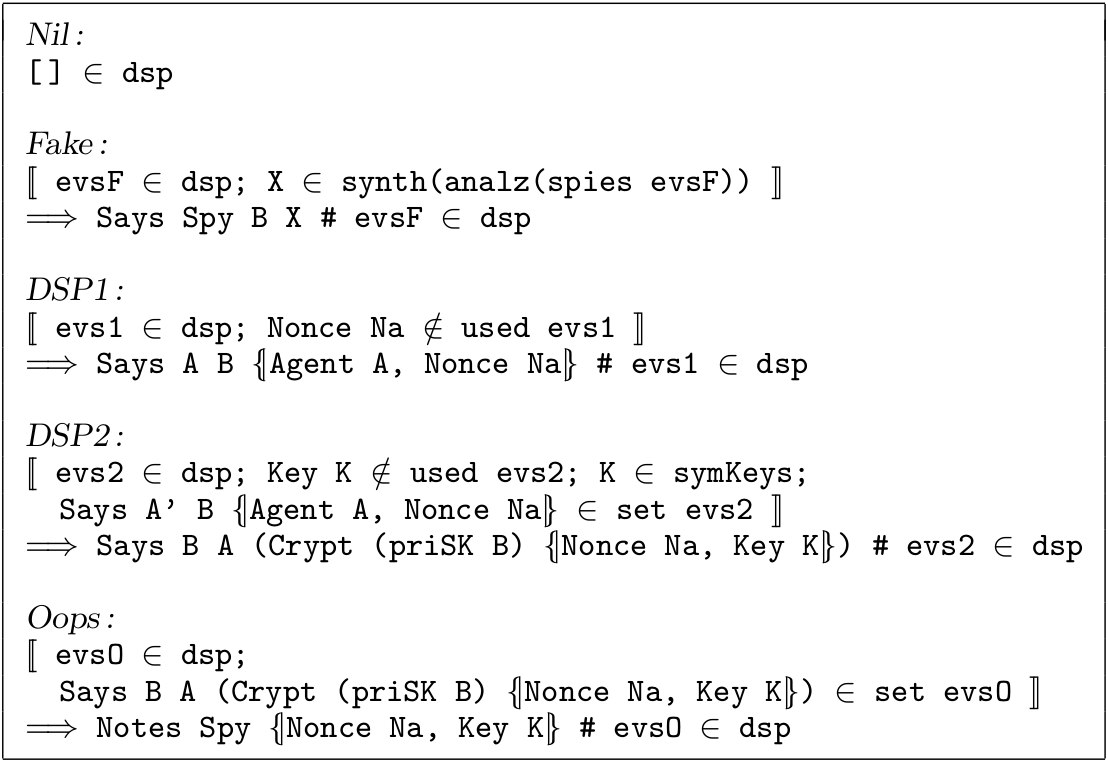
\includegraphics[width=0.8\textwidth]{img/prt-example-model}
  \caption{Formal model for the protocol displayed in Figure~\ref{prt:notation-example}. {\color{blue} essa imagem vai ser trocada para abarcar todos os eventos citados acima}}
\end{figure}

Using this model, the great majority of possible traces can be derived, but not every conceivable one, since the model should impose some restrictions on traces.





\section{Goals Verification}
Security protocols have technical properties that are inherent to its system, outlining how peers should communicate and the protocol proceed. Meanwhile, other important security aspects, introduced in Chapter~\ref{chap:sec-protocols}, are another kind of features that should be part of such specifications, being them another crucial role.

When the protocol formal model is defined, its underlying characteristics are not explicit. We need to present them, precisely stating its form, and proving that are valid to the model, i.e.\ they hold in all conceivable trace. This is the \textit{goal verification} stage, where each desired protocol feature is modeled as a goal and formal proofs build their validation to the model. Goals are divided in types, concerning the protocol property scope.

At the end, we also try to show that \textit{goal availability} is present in the model. This property provides formal guarantees to the agents that a given goal is present in that model, even under a threat model. Hence, this agents are assured that the protocol is reliably faithful to what it intends to offer.



\subsection{Reliability}
Reliability relates to how close a model is to the system it is representing. Note that such crucial property may not be really related to the security protocol goals but to system goals itself. As a result, the number of reliability theorems may vary from a protocol to another.

However, some basic properties, which are common for many protocols, are already defined and likely to be used in new formalizations. Some of them may seem obvious, but are important for formal systems. As examples, we can cite the idempotence of \texttt{analz} operator, fresh keys and session keys proper distinction, and the certainty of messages composition correctness.

The theorems of this class are easy to proof. They mainly use induction and simplification as its main proof strategy. Providing such goals gives us assurance that our model is reliable to the real world.



\subsection{Regularity}
The regularity lemmas are facts that can be proved from any message that appears in the traffic. Such properties may be applied to specific protocol goals, but some other broader properties can be guaranteed using them.

For example, regularity lemmas hold for long-term keys which can never be sent through the channel, since they are never meant to be used over the network, just in a agent local context. Therefore, it such agent key is seen in the traffic it is easy to derive that this agent is compromised, as stated below.

\begin{center}
  \texttt{Key} (\(shrK\ A\)) \(\in \) \texttt{parts} (\(knows\) \texttt{Spy} \textit{evs}) if and only if \(A \in bad\)
\end{center}



\subsection{Confidentiality}
Holding confidentiality in a protocol can be simply translated as to preventing the disclosure of certain messages to the Spy, that is, a message \(X\) cannot belong to the Spy knowledge set. Since messages are usually protected by encryption, this property is highly related to the use of cryptographic keys.

Precisely, the confidentiality of such keys is a major issue for the protocol confidentiality, specially session keys, because if the Spy obtains them, all messages encrypted under these keys could be easily acquired and altered by her. Hence, given a key \(K\), we have to be certain that at the end of all traces the key does not belong to the Spy knowledge set, as defined below.

\begin{center}
  \(\texttt{Key}\ K \notin \texttt{analz}\ (knows\ \texttt{Spy}\ evs)\)
\end{center}

Note that if \(K\) is encrypted with some other private key of an agent, the latter cannot be part of the compromised agents set. Otherwise, the Spy could easily retrieve the key from the compromised agent, obtaining the session key and further messages. Confidentiality is also interesting for nonces, which are commonly used assuring authenticity, computing checksum and other operations.



\subsection{Unicity}
The creation of fresh components in protocol is vastly used. It is seen in the production of session keys, nonces and other entities and they are mostly used for a single session, identifying it. Therefore, providing freshness in a protocol resembles unicity, a concept that establishes bounds between a message and its fresh components.

More precisely, if two events contain the same fresh message component, then they must be identical. Further, events containing fresh message components cannot occur more than once, otherwise they violate the unicity concept. Such lemmas are deeply explore when protocols apply the use of nonces and timestamps.

A formalization for this definition prompted the creation of a new predicate in Isabelle/HOL \textit{Auth} library, the \texttt{Unique} predicate. It takes an event and a trace as parameters, holding if the given event is unique in the given trace. Such formalization is crucial for detecting replay attacks over traces.



\subsection{Authenticity}
This property can also be read as legitimacy. In the method, the guarantee of a message's authorship is presented as synonym of integrity, since if the message is unaltered (integrity), then the authorship must be preserved. Even if the Spy intercepts the message and them relays it to the recipient, if integrity is preserved, then legitimacy is still preserved, since the Spy acted as a channel relay.

As a result, it is important that the message's author does not belong to the compromised agent set. Conversely, any messages sent by him would be compromised as well and authenticity would not hold. Such concept may seem obvious for integrity matters, but it is important to enforce the authorship interest. Therefore, both properties are attached during our verifications.



\subsection{Authentication}
As discussed in Section~\ref{sec:protocols:auth}, authentication may assume many properties. Supposing an initiator \(A\), who completes a protocol session with a responder \(B\). In this run, authentication may be translated as:

\begin{enumerate}
  \item \textbf{Aliveness of B}, meaning that \(B\) has been running the protocol;
  \item \textbf{Weak agreement of \(B\) with \(A\)}, meaning that \(B\) has been running the protocol with \(A\);
  \item \textbf{Non-injective agreement of \(B\) with \(A\) on \(H\)}, meaning a weak agreement of \(B\) with \(A\), considering the set \(H\) of messages components;
  \item \textbf{Injective agreement of \(B\) with \(A\) on \(H\)}, meaning the non-injective agreement of \(B\) with \(A\), using the set \(H\) of message components, where \(B\) did not respond more than once on each session with \(A\).
\end{enumerate}

The Inductive Method does not provide formalisms to reason about the fourth point. Although, it is claimed on~\cite{Bella2007} that such formalization can be easily constructed by simply verification of repetition of a given event \textit{ev} in the analyzed trace, restraining the agents to single responses. However, the method mainly tries to provide models that are more permissive as possible, stating that any message could be repeated over traces with no harm to model.

Specifically, non-injective agreements have a bigger focus. Regarding key distribution protocols, such property applied to session keys establishes a trust relation between the two agents, with a given key as a validation of such relationship, since both agents are uncompromised.

Eventually, \textbf{key distribution} becomes a major goal to be checked. Since this concept is related to the agreement of two agents in a mutual secret, it is stated in~\cite{BellareRogaway93} that this property is, indeed, stronger than authentication and thus, authentication itself relies on key distribution. Additionally, the authors of the Inductive Method proves that if authentication holds, so does key distribution, specifically non-injective agreement on a session key.



\subsection{Goal Availability}
The concept of goal availability is one of the main contributions in the work of G.~Bella~\cite{Bella2007}. In summary, it establishes a formal guarantee that the protocol model could met a given goal and, once this is true, the validity of such goal can be applied to all peers within their assumptions. If such property holds to the model, but cannot be checked by the peers, it is argued that this goal is not available and thus, not fully assured.

Also, goal availability is closely related to the threat model considered by the protocol and its peers minimal trust. Considering the former, our the adopted model is the Dolev-Yao, faithfully implemented by the Inductive Method using abstractions described in Sections~\ref{ssec:threat-model} and~\ref{ssec:operators}. If a different threat model is considered, important aspects of the model context are also altered, which may change the validity of previous goals.

\textit{Minimal trust} concerns facts that agents must assume true, due to inability to verify them, in order to check a protocol guarantee from their point of view. Precisely, agents can only verify what they send and receive from the network, having no guarantees at all about other peers. Likewise, agents cannot state if they are compromised. Therefore, they must take such facts as true, in order to establish a suitable set of clauses to attest some goal. We formally define minimal trust below.

\begin{definition}
  Let \(\mathcal{P}\) be a security protocol, \(P\) be a formal model for \(\mathcal{P}\), and \(A\) be an agent's name. The \textit{minimal trust} of \(A\) is the set of environmental facts formalised in \(P\) whose truth values \(A\) needs to know but can never verify.
\end{definition}

Having notion of what agents can verify, an \textit{aplicable guarantee} can be defined.

\begin{definition}
  Let \(\mathcal{P}\) be a security protocol, \(P\) be a formal model for \(\mathcal{P}\), and \(A\) be an agent's name. A formal guarantee in \(P\) is \textit{applicable} by \(A\) if it is established on the bais of assumptions that \(A\) is able to verify in \(P\) within her minimal trust.
\end{definition}

In these previous definitions, it is clear that guarantees that are applicable by an honest agent \(A\) are not necessarily applicable by another honest agent \(B\). Hence, this strengths the argument that only proved assumptions concerning protocol messages, specially the ones related to the agent, are the valid formal guarantees for a given protocol goal.

Finally, the definition of available goal can be made. The principle should be used to guide the formal proofs about goals. As a result, whenever a goal is not available to some peer, it is not guaranteed at that model and so, it does not hold for the given protocol.

\begin{definition}
  Let \(\mathcal{P}\) be a security protocol, \(P\) be a formal model for \(\mathcal{P}\), \(g\) be a goal for \(\mathcal{P}\), and \(A\) be an agent's name. The goal \(g\) is \textit{available} to \(A\) in \(P\) if there exists a formal guarantee in \(P\) that confirms \(g\) and that is applicable by \(A\) in \(P\).
\end{definition}
